\begin{figure}
\begin{center}
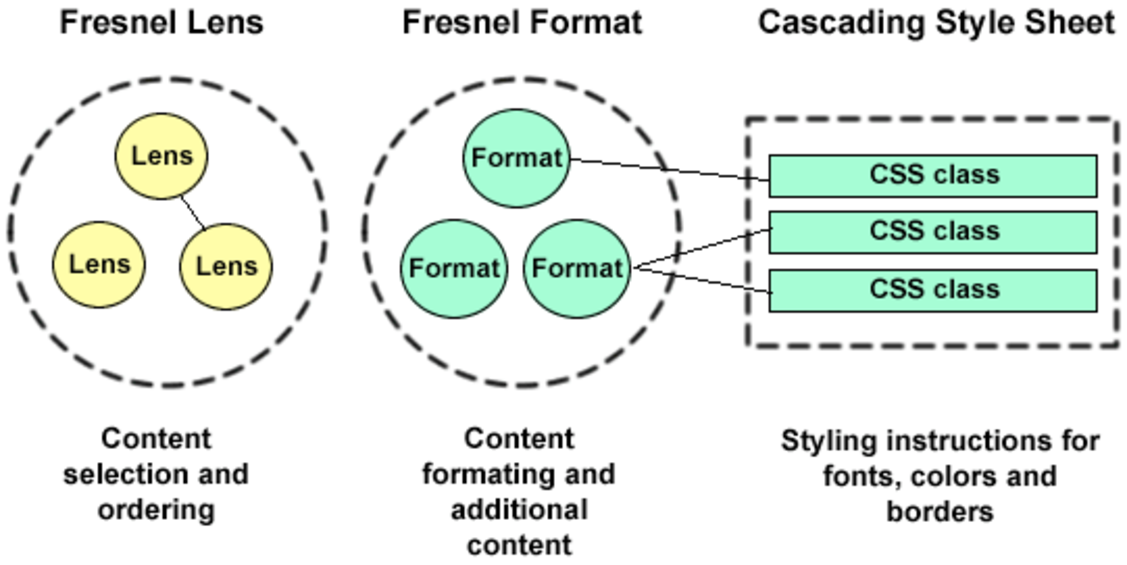
\includegraphics[width=8cm]{overview.pdf}
\caption{Fresnel foundational concepts}
\label{foundationalConceptsFig}
\end{center}
\end{figure}


%--------------------------------------------------------------------
\section{Fresnel Core Vocabulary Overview}
\label{fresnelov}

Fresnel is an RDF vocabulary, described by an OWL ontology \cite{fresnel05}. Fresnel presentation knowledge is thus expressed declaratively in RDF and relies on two foundational concepts: {\em lenses} and {\em formats} (see Figure \ref{foundationalConceptsFig}). Lenses specify which properties of RDF resources are shown and how these properties are ordered while formats indicate how to format content selected by lenses and optionally generate additional static content and hooks in the form of CSS class names that can be used to style the output through external CSS style sheets.

Figure \ref{exampleFig} shows a simple lens and associated formats used to present information about a person described with the FOAF vocabulary \cite{foaf}. This figure also shows a hypothetical rendering of such a resource, as an Horus \cite{horus} or Longwell-like browser could produce. Examples use the Notation 3 syntax \cite{N3}.

\begin{figure}
\begin{center}
\begin{tabular}{lp{4.5cm}}
\begin{small}
\begin{tt}
\begin{tabular}{ll}
(1) & :PersonLens a fresnel:Lens ;\\
(2) & ~~~~fresnel:classLensDomain foaf:Person ;\\
(3) & ~~~~fresnel:showProperties (\\
(4) & ~~~~~~~~foaf:name\\
(5) & ~~~~~~~~foaf:mbox\\
(6) & ~~~~~~~~foaf:depiction\\
(7) & ~~~~).\\
(8) & :nameFormat a fresnel:Format ; \\
(9) & ~~~~~~~fresnel:label "Name" ;\\
(10) & ~~~~~~~fresnel:propertyFormatDomain foaf:name .\\
(11) & :mboxFormat a fresnel:Format ;\\
(12) & ~~~~~~~fresnel:propertyFormatDomain foaf:mbox ;\\
(13) & ~~~~~~~fresnel:label "Mailbox" ;\\
(14) & ~~~~~~~fresnel:value fresnel:externalLink ;\\
(15) & ~~~~~~~fresnel:valueFormat [ fresnel:contentAfter "," ] .\\
(16) & :depictFormat a fresnel:Format ;\\
(17) & ~~~~~~~fresnel:propertyFormatDomain foaf:depiction ;\\
(18) & ~~~~~~~fresnel:label fresnel:none ;\\
(19) & ~~~~~~~fresnel:value fresnel:image .\\
\end{tabular}
\end{tt}
\end{small}
&
\begin{picture}(45,0.1)(0,0)\put(-27,65){\makebox(0,0){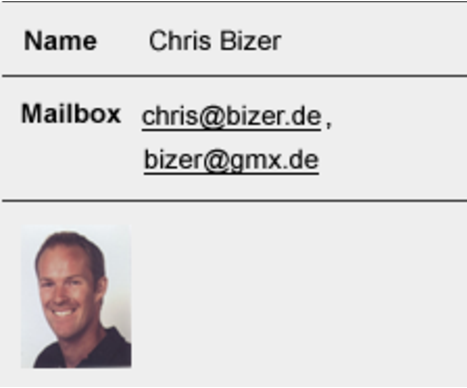
\includegraphics[width=4.2cm]{boxmodelexampleoutput.pdf}}}\end{picture} \\
\end{tabular}
\caption{A lens and some formats for presenting instances of class \rdf{foaf:Person}}
\label{exampleFig}
\end{center}
\end{figure}

\vspace{-1.5cm}

\subsection{Content selection}

The domain of a lens indicates the set of resources to which a lens applies (line 2). Property \rdf{showProperties} is used to specify what properties of these resources to show and in what order (lines 3-7). In this example, the values of both \rdf{classLensDomain} and \rdf{showProperties} are basic selectors, which take the form of plain URIs (represented here as qualified names), respectively identifying the class of resources and property types to select. More complex selection expressions can be written using either FSL or SPARQL (see section \ref{selectors}), making it possible to associate lenses with untyped RDF resources, which do occur in real-world models since \rdf{rdf:type} properties are not mandatory. Format domains can also be specified with one of these three solutions.

Fresnel Core provides additional constructs for specifying what properties of resources to display. The special value \rdf{fresnel:allProperties} can be used to avoid having to explicitly name each property that should be displayed. This value is also useful when the list of properties that can potentially be associated with resources handled by a lens is unknown to the lens' author but should nevertheless be displayed. When it appears as a member of the list of properties to be shown by a lens, \rdf{fresnel:allProperties} designates the set of properties that are not explicitly designated by other property URI references in the list, except for properties that appear in the list of properties to hide (\rdf{fresnel:hideProperties}). The extended lens vocabulary defines two other constructs to handle the potential irregularity of RDF data stemming from the fact that different authors might use similar terms coming from different vocabularies to make equivalent statements. Sets of such similar properties can be said to be \rdf{fresnel:alternateProperties}. For instance, \rdf{foaf:name}, \rdf{dc:title}, and \rdf{rdfs:label} could be considered by a lens as giving the same information about resources. A browser using this lens would then try to display the resources' \rdf{foaf:name}. If the latter did not exist, the browser would look for \rdf{dc:title} or \rdf{rdfs:label}. The second construct, \rdf{fresnel:mergeProperties}, is used to merge the values of related properties (e.g. \rdf{foaf:homepage} and \rdf{foaf:workHomepage}) into one single set of values that can later be formatted as a whole.

The presentation of property values is not limited to a single level, and recursive calls to lenses can be made to display details about the value of a property. Inserting the following lines in Figure \ref{exampleFig} between lines 6 and 7:\\
\begin{small}
\begin{tt}
\begin{tabular}{ll}
(6a) & ~~~[rdf:type fresnel:PropertyDetails ;\\
(6b) & ~~~~fresnel:property "foaf:knows[foaf:Person]"$^{\wedge\wedge}$fresnel:fslSelector;\\
(6c) & ~~~~fresnel:sublens :PersonLabelLens]\\
\end{tabular}
\end{tt}
\end{small}
\\tells the browser to render values of the property \rdf{foaf:knows}, which must be instances of \rdf{foaf:Person}, using another lens (\rdf{PersonLabelLens}). Infinite loops cau\-sed by recursive calls to the same lens are prevented by a closure mechanism.

\subsection{Content formatting}

The representation of selected information items mainly depends on the browser's representation paradigm (e.g. nested box layout, node-link diagrams, etc.) which defines the rendering method. The final rendering can be further customized by associating formatting instructions with elements of the representation.

Formats apply to resources, or to properties and their values, depending on the specified domain. The three example formats of Figure \ref{exampleFig} apply respectively to the properties \rdf{foaf:name}, \rdf{foaf:mbox} and \rdf{foaf:depiction} (lines 10,12,17). Formats can be used to set properties' labels (lines 9, 13, 18) and to indicate how to render values. For instance, line 14 indicates that \rdf{foaf:mbox} values should be rendered as clickable links (email addresses). Values of \rdf{foaf:depiction} should be fetched from the Web and rendered as bitmaps (line 19). Fresnel also defines default display methods in case such indications are not given by a format.

Property values can be grouped, and additional content such as commas (line 15) and an ending period can be specified to present multi-valued properties. CSS class names can also be associated with the various elements being formatted. These names appear in the output document and can be used to style the output by authoring and referencing CSS style sheets that use rules with the same class names as selectors.
